\documentclass[../main.tex]{subfiles}
\graphicspath{ {../img/} }


\begin{document}


	\chapter{Part 2}


	\section{Why Rust?}


    Rust is a multi-paradigm low level programming language which emphasizes memory safety, strict types and high performance. 
    Despite its novel features(and associated learning curve), such as variable ownership and its ommission of a null variable, it is already a loved language among developers, which forces the developer to write safer and more performant code.
    Despite it lacking as many footguns as C/C++, it allows a great deal of control over what happens in a program. 
    Though young, Rust is seen as the spearhead for the languages of the future, looking to replace C++ as the dominant low level language. 
    Rust has been added to the Linux kernel, currently the only language to accompany C in this domain, and is being picked up by even the largest companies, such as Google. On the opposite side of the spectrum, hackers have begun writing in Rust, due to its aforementioned strengths and the current inability for malware scanners to detect threats in the binary[reference]. 
    All of these reasons combined form our argument for learning Rust, which is what we had to do for this project.

	\vspace{10pt}

	\section{Flow of the program}

    Let's Now analyse our rust code to have a better understading of the communications in our botnet.
	\vspace{10pt}

	\subsection{Server code}

    \# server/src/main.rs

    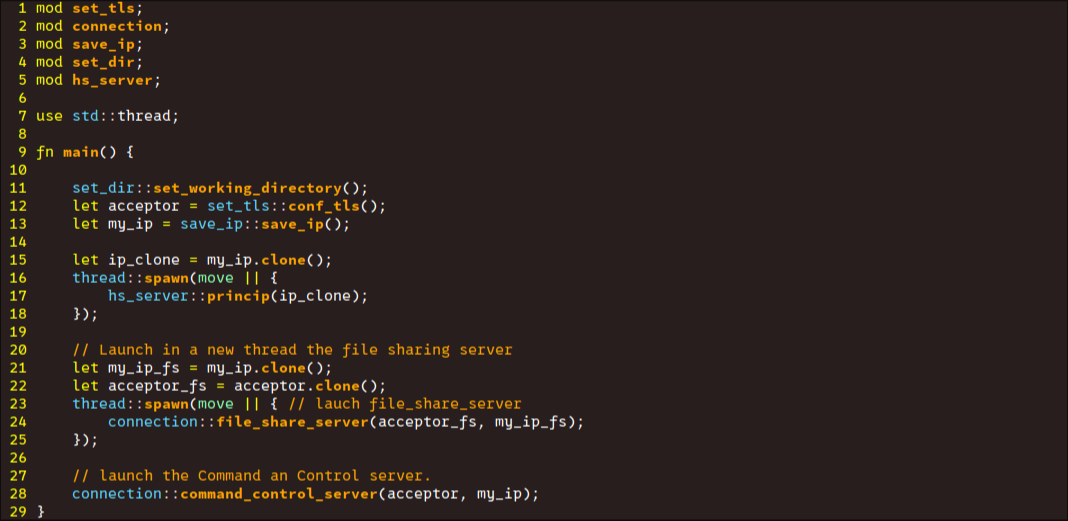
\includegraphics[width=450pt]{server_main.png}

    Here, we can see that first, we import line 1-5 different modules that we have written, to help us writting all together on the code at the same time.
    Then, line 7, we import thread.
    The main function begin, and immediately, we set the working directory, to where the binary is.
    After that, we create the acceptator, save the server ip address, and give it in a different thread to the hs\_server, the hacking server, which will transform the victim to a bot.
    Now, we are to the last part of the server.
    It generate the file sharing server in another thread, and then, wait for connection for the command and control server.

    
	\vspace{10pt}

	\subsection{Client code}

    Now, let's talk about the client's code.

    \# client/src/main.rs

    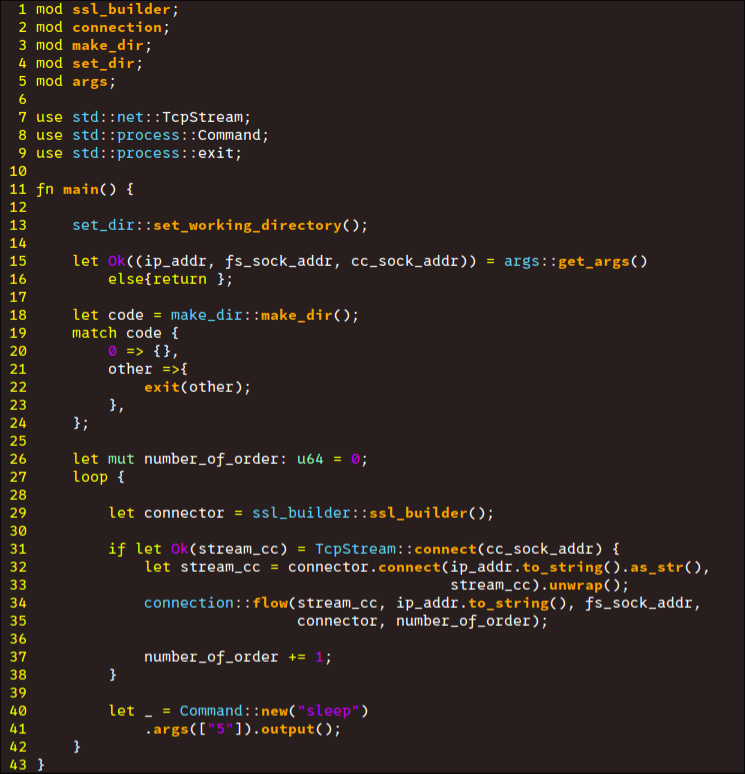
\includegraphics[width=450pt]{client_main.png}

    The begining of the main is the import of different functions.
    Then, it imports TcpStream, to make the stream object, command, to run system command, and exit, to exit in case there is a problem.
    Then, the main start, the working directory is set where the binary is, it makes all the nessecarry directory, like www, downloaded or conf, and exit in case of an error.
    Then, it makes the stream with the CC server, and launch the flow. 
    It counts the number of times it loops, that usefull to know if it's the first time or not that it's connect to the server, adn then to ask for order1 or order2.
    After each successful connection, it's wait for 5 seconds, before launching the next connection.


    \# client/src/connection.rs

    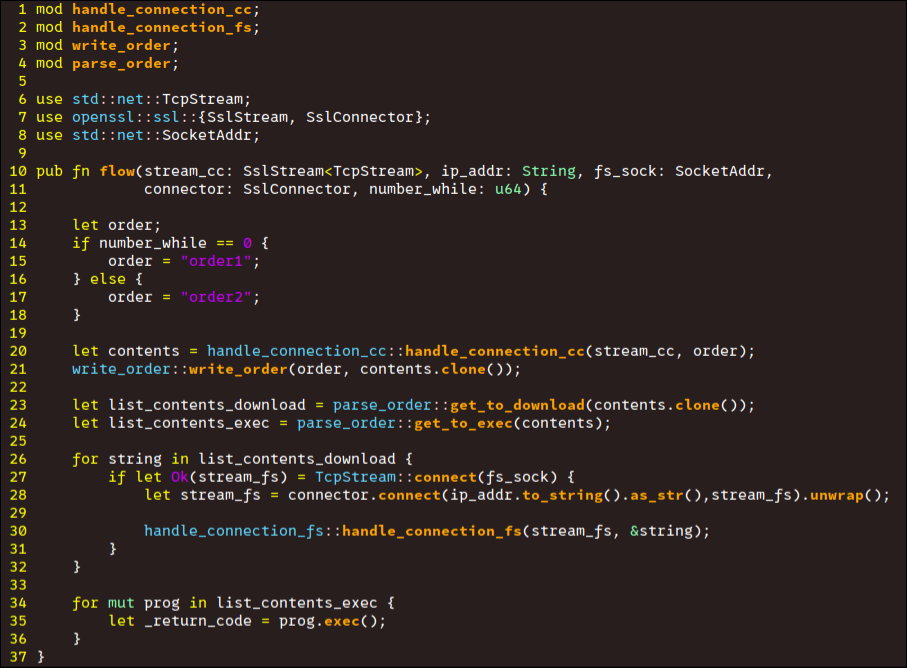
\includegraphics[width=450pt]{client_flow.png}

	\vspace{10pt}

	\section{Difficulties encountered while writting the program}



\end{document}
